\documentclass{article}
\usepackage{graphicx} % Required for inserting images
\usepackage{url}
\usepackage{hyperref}
%\usepackage{natbib}
\usepackage{verbatim}
\usepackage{natbib}
\usepackage{amsmath} 

\usepackage[letterpaper,top=3cm,bottom=3cm,left=4cm,right=4cm,marginparwidth=1.75cm]{geometry}

\begin{document}

\title{Higher Education Access Disparities in Portugal}
\author{Miguel Sousa Duarte\thanks{{\tiny{}Department of Economics, Copenhagen Business School. \textbf{E-mail}: \url{msd.eco@cbs.dk}.}},
Vicente Conde Mendes\thanks{{\tiny{}École Polytechnique Fédérale de Lausanne. \textbf{E-mail}: \url{vicente.c.mendes@gmail.com}.}}\\}

\date{\today}

\setlength{\parskip}{1em}
\maketitle
PhD studies progress: 1st year in a 3-year programme.

Commitment to research proposal: My PhD specialization is Pension Economics. Therefore, I might be unable to make this one of the chapters, for lack of connection to the main topic. Nonetheless, I plan to take the project through to its end.

I would greatly appreciate feedback!

I have already started working on this project. I have access to data on internal and external grades. I am waiting for approval on getting data on students' public university choices.


\newpage

\section{Introduction}
While private school students tend to outperform their public school peers on both internal grades and national exams, they also experience greater grade misalignment — meaning the gap between their school-given grades and their exam results is wider. If university admissions rely on inflated internal grades, private school students may benefit disproportionately. In this study, we quantify grade inflation across schools and simulate an alternative admissions process that corrects for these disparities, shedding light on the role of grade inflation in shaping access to higher education.

In Portugal, 25\% of high school (HS) students attend private institutions (Pordata, 2022). In general, private HS, which can select which students to admit into their alumni, are fully-funded by the tuition they charge their students. As such, on average, students in private HS come from a more privileged socioeconomic background. 

In Portugal, graduation from high school is conditional on passing standardized national exams on some of the subjects the students took during HS. 

Private HS students achieve higher grades both on school-internal grading and on National Exams (NE) when compared to public HS students. This can be due to several reasons, among them, 1) private HS students' innate ability is better; 2) private HS students have access to better outside-of-the-classroom resources; 3) the education provided by private schools is better. Reason 1) may cause backlash but it is not implausible that ability of parents is correlated with ability of children and that ability of parents is correlated with income of parents. Reason 2) derives from the plausible assumption that having the means and willingness to pay for private education positively correlates with having the means and willingness to pay for tutoring. As for reason 3) it is widely recognized in Portugal that private HS tend to provide a better education than their public counterparts - even though reasons 1 and 2 may contribute towards the overall societal perception of the gap in education quality.
Nonetheless, it seems agreeable to conclude that private HS students in Portugal are privileged. 

Private schools' students score, on average, 4.1 points below on their national exams compared to their school-given grade (Figure \ref{fig: InflationBySchoolType}). For public schools, this gap is of 3.7 points. In fact, as stated by \cite{sapo2024}, the ten 10 HS with the greater difference between internal grading and NE grade are private.
If national exams are a good measure of true ability, then private schools inflate their students' grades by 10\% than public schools. This provides an unfair advantage to private HS students.

\begin{figure}[ht]
  \centering
  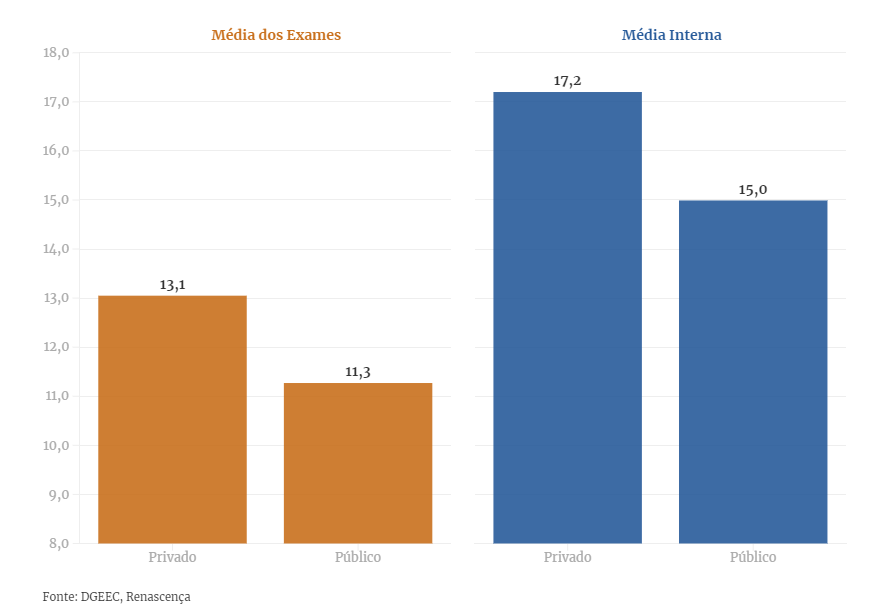
\includegraphics[height=4.3cm, keepaspectratio]{Figures/InflationBySchoolType.png}
  \caption{Grade Misalignment by School Type \citep{sapo2024}}
  \label{fig: InflationBySchoolType}
\end{figure}
%add source



\cite{nata2014unfairness} group students by the 1-step range grade that they scored on the NE, and then plot for each group of schools the mean of the misalignment. The plot is brought to you on Figure \ref{fig: Inflation_Nata}. It is clear that for each class of score on NE, the private high-schools always have a greater differential. This is indicative of some inflation performed by private schools. 


\begin{figure}[ht]
  \centering
  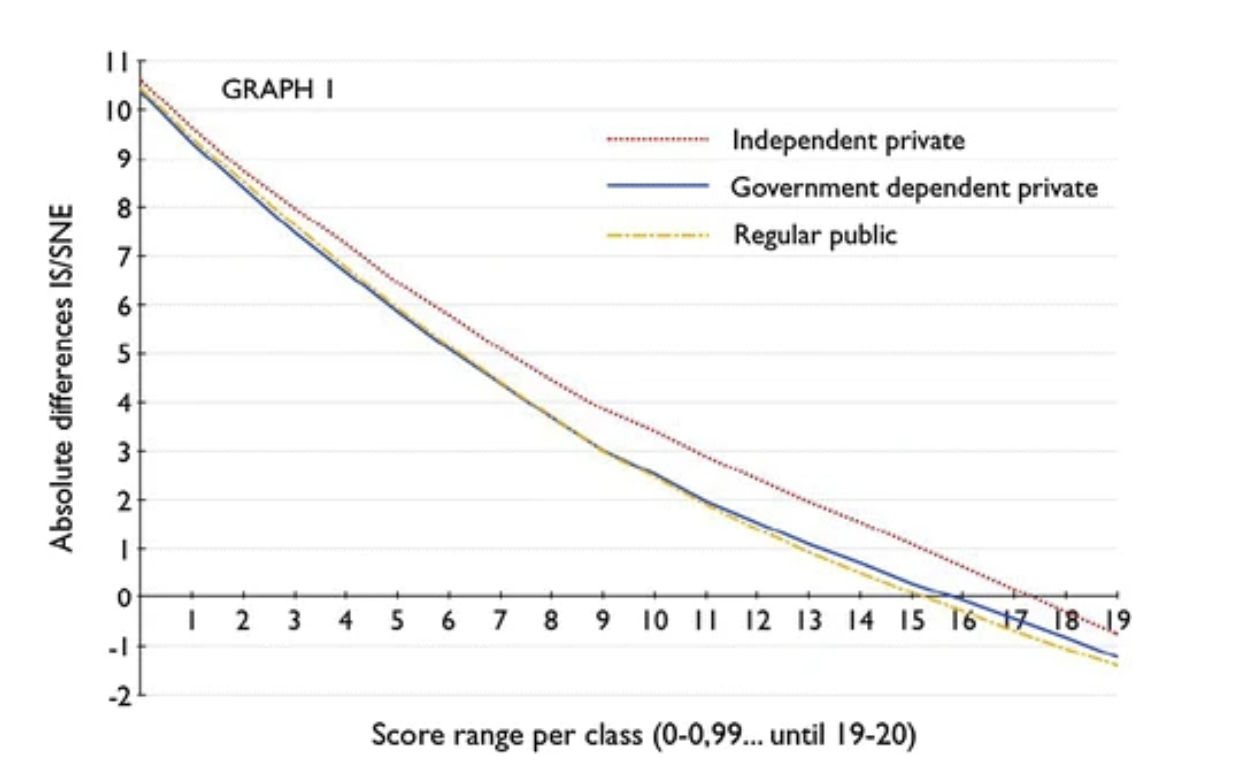
\includegraphics[height=7cm, keepaspectratio]{Figures/Inflation_Nata.png}
  \caption{Grade Misalignment plotted against NE grade \citep{nata2014unfairness}}
  \label{fig: Inflation_Nata}
\end{figure}



\section{Literature Review}

\cite{nata2014unfairness} find that independent private schools inflate their students’ scores when compared to both public and government-dependent private schools. The authors further find that inflation is higher where scores matter most: in the competition for the scarce places available in public higher education. The authors provide descriptive statistics of the grade inflation, without laying out but a small intuition into the implications for access to higher education. We propose an empirical exercise through which the process of accessing higher education is recalculated.

\cite{silva2025public} build on the analysis performed by \cite{nata2014unfairness} by structuring a multinomial logit that models the probability of grade inflation according to school type and some other controls. Though we do not follow their regression, their considerations for potential grading bias are valuable.


\section{Institutional Details}
The admission process of students to public higher education in Portugal is centralized. Students rank their preferred university-programme pairs of choice in a list with a maximum of 6 elements. Admission follows a deferred acceptance algorithm exclusively dependent on the GPA with which the student concluded High School and on the grades scored on the NE. Generally, the application grade is the arithmetic mean of the school-given internal grade and the grades scored on the NE relevant for the Bachelors programme (exact proportion and which NE are relevant are defined by the university). The key factor here is that the schools' internal grading play a relevant role in university application GPA, in a system in which this is the only qualifying mechanism.

Students must take a set of NE (provided and graded by the central government) that depends on which track of studies the student has chosen for the 3 years of HS studies. Students are able to voluntarily sign up for additional exams (if for example, they are aiming for a drastic change of subject going into university and therefore need an exam for university admission that was not part of the mandatory ones of their HS study track)

Note that the final internal grade is also dependent on national exams. By government rule, for each subject, the internal grade is 70\% teacher's grade and 30\% national exam grade (which helps attenuate the possible perverse effect we study here). You can visualize the rules for GPA computation in Figure \ref{fig: GradeComputationPortugal}.

\section{Data}
Our data is sourced from the Directorate-General for Statistics of Education and Science (in Portuguese, DGEEC) which has data on all HS-related grades: both internal and national exams. The choices of HS graduates for public Higher Education made on the National Access Contest (in Portuguese, CNA) and are accessed via DGEEC too.

The dataset on HS-related grades displays the school attended, the grades attributed internally and the grades scored in the NE.
The dataset on the public university access (CNA) has data on the (up to) six options HS graduates have ranked in their university application. 
The dataset on public higher education has the university and programme in which each of the students is enrolled in, in each year.
A personal identifier number allows for merging the datasets. 
Demographic variables including age, country of origin and parental occupation can be used as controls.

Internal grading (CIF) is on a scale of 0-20, where as national exam grade (CLASS\_EXAM) is on a scale of 0-200. They are easily comparable and additive if we multiply the former by factor 10. Note, however, that the exam grade is more discrete and allows for more differentiation than internal grading. 

The dataset on the NE grades actually has the grade obtained after the exam, and also the final grade after possible revisions of the grade. We pick the latter and abstract from the fact that there may be a tendency for either public or private HS students to be more likely to ask for a revision of their grade. In spite of the financial cost associated with it, given that, when asking for a revision, the student risks ending up with a lower grade than attributed originally, we find this to be a fair assumption.

The dataset could be enriched by linking it to labour market outcomes. This would require engaging with other governmental bodies other than DGEEC. Data in Portugal is not as centralized as in the Scandinavian countries and to the best of our knowledge, no one has done this linkage before for Portuguese data, which makes the task both harder and more valuable.

\section{Empirical Work}
We start by building upon the analysis by \cite{nata2014unfairness} in that we look at how the internal grade - external grade misalignments differ across different types of schools. We start by understanding the degree of recidivism of schools: are there some schools that consistently exhibit a pattern of higher differential?
We also explore the distribution of these differentials, within private and public schools. We get inspiration from the graph of \cite{sapo2024} that is displayed on Figure \ref{fig:InflationBySchool_Grouped}. 

\begin{figure}[ht]
    \centering
    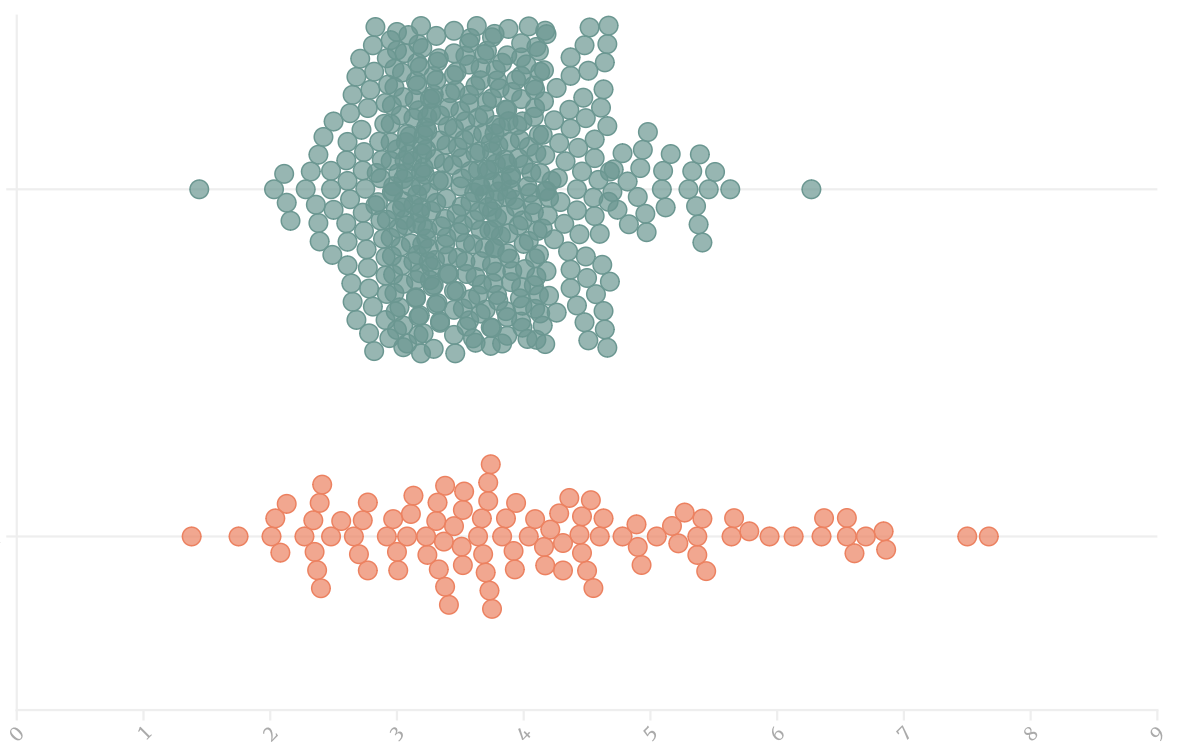
\includegraphics[width=0.5\linewidth]{Figures/Screenshot 2025-03-07 at 19.18.55.png}
    \caption{Grade Misalignment by School and School Type \citep{sapo2024}}
    \label{fig:InflationBySchool_Grouped}
\end{figure}


Blue dots are public HS, and orange ones private. The misalignment is generalized for both types of school. The means are not so different across groups, however, we see that across private high-schools, the variance of the differential is much higher than across public schools. The problem here we hypothesize is the orange dots to the right. These private schools inflate their grades so much, that their students take away desirable university spots from public HS students. Our intuition is that the students in the orange-dot schools further to the left actually do not experience unfairness compared to say, a student experience the average misalignment across the blue dots. These orange-dot schools already award fairly high grades to the (often high ability) students that in them are enrolled, and therefore the upper bound is having an effect here.

There are two policy changes that we wish to explore. The inspiration for these lies on the statement of \cite{nata2014unfairness} that it seems reasonable to assume that grade inflation might be even higher where no comparative scrutiny can be effectively carried out.

\begin{itemize}
    \item In the 2018/2019 school year, Physical Education became part of the HS GPA. Though this may require further fundament, we believe there is no reason to believe that private HS are more prone to physical activity, yet %need to back this with data
    they are awarded, on average, higher scores than students in public HS. What was the impact of the change in this policy? How much worse off did public HS students become?
    \item In the Covid period, rules regarding mandatory NE became more lenient: students only had to take exams they wanted to use for accessing Higher Education. The attenuating effect of the NE counting for the internal grade was therefore weaker during this period for some of the subjects. Furthermore, exams were easier, graded out of 20 but with 20+ possible points. A higher rate of students getting a perfect score puts more emphasis on internal grading in distinguishing the students. Both of these points are concerning. Though our external grading sample for comparison decreases, it may be useful to make a comparison across different year-cohorts in the same school to see whether teachers inflated grades further given that, during this period, there was no NE grade to compare the students' school performance to.
\end{itemize}


We now move on to the main exercise we propose doing: that of running the algorithm of public university admission for grades adjusted for school-subject-specific inflation.\footnote{Two clarifications are worth making. The first one is that we try to distinguish the terms "misalignment" or mark-up and "inflation" by stating that the difference between internal grade and external grade is the misalignment, and inflation is how a school's misalignment compares to others / the average. The second one is that we implicitly assume that individuals' true ability is perfectly represented by the grade scored in the national exam. Arguably, evaluating true ability via a single exam is set to be subject to some measurement error. %We later relax this assumption. %hopefully
}

The process, described analytically below, is as follows: for each subject with a national exam, we determine the average grade misalignment per school by comparing school-specific grades to the national average. Using this measure, we adjust each student’s internal grade for that subject by the difference between their school's misalignment and the average national misalignment (which is what we label inflation). The Adjusted Final Internal Grade is then computed by combining these adjusted grades for exam subjects with the original internal grades for subjects without a national exam.

\[
\text{Adj.Grade} = \text{Internal Grade} - \text{Subject School Specific Grade Inflation}
\]  

Let $n_{s,m,i}$ be the number of subject $m$ exams taken at school $s$ by student $i$, which we expect to be one! 
Let $n_{s,m}$ be the number of subject $m$ exams taken at school $s$.
Let $n_{s}$ be the number of exams taken at school $s$.
Note that $\sum^{M}_{m=1} n_{s,m} = n_s$. IG stands for internal grade and EG for external grade.


\[
\text{School \textit{s} Subject \textit{m} Student \textit{i} Mark-up} = IG_{s,m,i}-EG_{s,m,i}
\]

\[
\text{School \textit{s} Subject \textit{m} Average Mark-up} = \frac{\sum\limits_{i=1}^{n_{s,m}} (IG_{s,m,i}-EG_{s,m,i})}{n_{s,m}} 
\]


\[
\text{School \textit{s} Mark-up} = \frac{\sum\limits_{m=1}^{M} \sum\limits_{i=1}^{n_{s,m}} \left( IG_{s,m,i} - EG_{s,m,i} \right)}{n_{s}}
\]


%Let $n_{s,i}$ be the number of exams student $i$ takes at school $s$. Ideally, $s$ would be redundant in that student $i$ would only take exams in one school. Will have to look into students who decide to move schools in the last year of high school.

Then, we take take the country average of the mark-up on subject \textit{m}:

\[
\text{Cross-Country Subject \textit{m} Mark-up} = \frac{\sum\limits_{s=1}^{S} \text{Mark-up}_{s,m}}{S}
\]

Where S is the total number of schools in the country. % Do we need an adjustment for the size of the school?

\[
\text{Student \textit{i} Subject \textit{m} Adjusted grade} = IG_{s,m,i} + (\text{Mark-up}_{s,m} - \text{Country Mark-up}_{m} )
\]

Accounting for this adjustment, we simulate the application algorithm that allocates public university spots.
The main question we want to answer with this re-calculation is the following: Does the proportion of public high school students in high grade requirement courses increase upon this adjustment?

\section{Conclusion}
Our work is inspired by the unfair advantage that private HS students have in comparison to their public HS peers, when applying to Higher Education, due to more favourable internal grading, which is part of the university application GPA - the main factor for admission. These individuals also come from a more advantageous socioeconomic background and therefore get better support outside of the classroom.

Our contribution consists of adjusting the internal grades of students in accordance to how their school's misalignment between internal and external grade deviates from the country's average. Then, we re-run the algorithm for the university assignment and compare the adjusted outcome to the original governmental one.

If the most able students are not getting the most challenging spots, then there is room for inefficiency. A measurement of the welfare impact of this sub-optimality is not provided in this paper. We are more concerned with the unfairness that a certain group of students may be exposed to. In particular, we are interested in how many students, with which backgrounds and high schools are being affected by other schools' inflation. Quantifying the economic impact on these individuals would have been an interesting addition that requires further data and that we, therefore, leave for further research. All in all, we believe that shedding light on the grade misalignment discrepancies across high schools is useful for society and we innovate by simulating the university application process with adjusted grades.

\bibliographystyle{apalike}
\bibliography{references}

\newpage
\appendix
\section{Appendix}

\renewcommand{\thefigure}{A\arabic{figure}} % Change figure numbering to A1, A2, etc.
\setcounter{figure}{0} % Reset figure counter

\begin{figure}[ht]
  \centering
  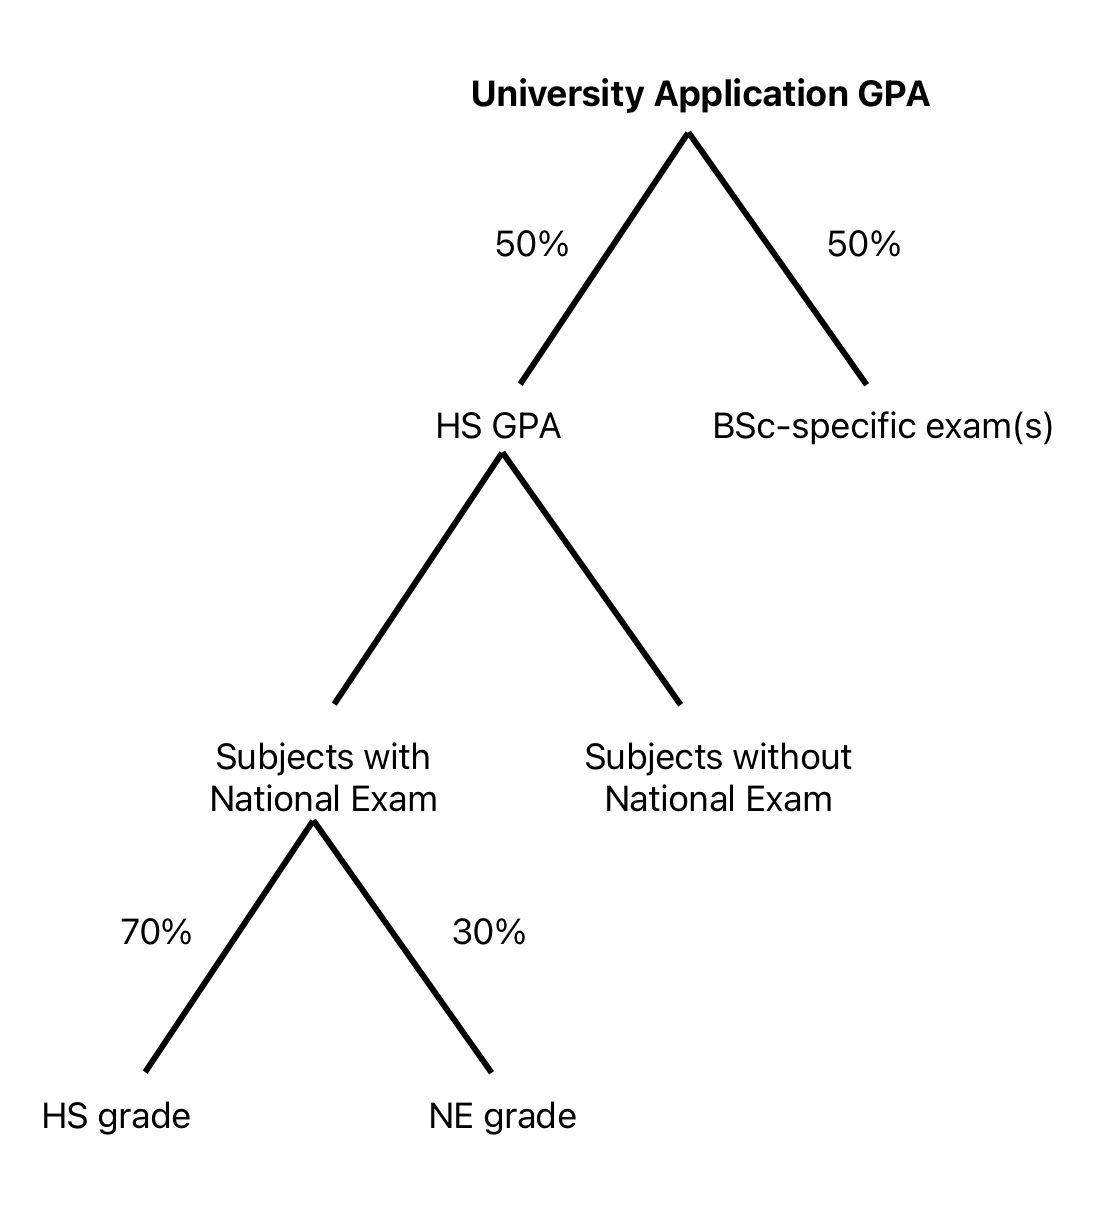
\includegraphics[height=10cm, keepaspectratio]{Figures/GradeComputationPortugal.jpeg}
  \caption{GPA Computation Rules in Portugal}
  \label{fig: GradeComputationPortugal}
\end{figure}

\end{document}